\documentclass[10pt,aspectratio=43,mathserif, notes]{beamer}		
%设置为 Beamer 文档类型,设置字体为 10pt,长宽比为16:9,数学字体为 serif 风格, 带有注释

%%%%-----导入宏包-----%%%%
\usepackage{ctex}			 %导入 ctex 宏包,添加中文支持
\usepackage{xeCJK}
\usepackage{amsmath,amsfonts,amssymb,bm}   %导入数学公式所需宏包
\usepackage{color}			 %字体颜色支持
\usepackage{graphicx,hyperref,url,pgf}
\usepackage{pgfpages}	
\usepackage{ccnu}			%导入 CCNU 模板宏包
%%%%%%%%%%%%%%%%%%

\setsansfont{Helvetica.otf} 							%Windows和Mac OS下都可用
%\setsansfont{Times New Roman}
%\setCJKmainfont{Hiragino Sans GB W3}    	          %仅Windows可用
%\setCJKmainfont{Songti SC}								%仅Mac OS下可用

\beamertemplateballitem		%设置 Beamer 主题

%\setbeameroption{show notes on second screen=right} % 用于双屏显示notes

\CTEXoptions[today=old]     % 使日期显示为英文格式

\AtBeginSection[]
{
  \begin{frame}<beamer>
    \frametitle{\textbf{Outline}}
    \textbf{\tableofcontents[currentsection]}
  \end{frame}
}


%%%%----首页信息设置----%%%%
%\title[Synaptic Plasticity and Pattern Interference]{\fontsize{13pt}{18pt}\selectfont {Synaptic Plasticity and Pattern Interference in Liquid State Machine for Time Series Classification}}
%\subtitle{\fontsize{9pt}{14pt}\selectfont \textbf{Infrastructure and Algorithms}}		
\title[Synaptic Plasticity and Separative Responses]{\fontsize{13pt}{18pt}\selectfont {Synaptic Plasticity and Separative Responses in Liquid State Machine for Time Series Classification}}
\subtitle{\fontsize{9pt}{14pt}\selectfont \textbf{Infrastructure and Formal Definition}}		
%%%%----标题设置

\author[Ryan Zhou]{Ryan Zhou\\\medskip
  {\small zhouy@mail.neu.edu.cn}}
%%%%----个人信息设置

\institute[SAPI]{
  State Key Laboratory of Synthetical Automation for Process Industries (SAPI)\\
  Northeastern University}
%%%%----机构信息

\date[\today]{
 \today}
%%%%----日期信息


\begin{document}
%---------------------------------------------------
\begin{frame}
\titlepage
\end{frame}				%生成标题页



\section*{Outline}
%---------------------------------------------------
		\begin{frame}
		\frametitle{\textbf{Outline}}
		\textbf{\tableofcontents}
		\end{frame}				%生成提纲页

\section{Introduction}
%---------------------------------------------------
		\begin{frame}
			\frametitle{\textbf{Introduction}}
            \noindent\textbf{Background}\\
                 \textcolor[rgb]{1.00,0.00,0.00}{Spiking Neuron Networks (SNNs)} are often referred to as the $3^{rd}$ generation of neural networks. Highly inspired from natural computing in the brain and recent advances in neurosciences, they derive their strength and interest from an accurate modeling of synaptic interactions between neurons, taking into account the time of spike firing.\cite{RN158,RN85,RN113}
        \end{frame}

%---------------------------------------------------
		\begin{frame}
            \noindent\textbf{Motivation}
                \begin{itemize}
                    \item The model is \textcolor[rgb]{1.00,0.00,0.00}{more biological plausible} than Artificial Neural Network to simulate the mechanism of \textcolor[rgb]{1.00,0.00,0.00}{brain-like Computing}.
                    \item Not only traditional learning rules but also Many \textcolor[rgb]{1.00,0.00,0.00}{bio-inspired learning rules} are available for SNN without the limitation of the vanishing gradient.
                    \item Information is processed by spikes in SNN, which is consider as \textcolor[rgb]{1.00,0.00,0.00}{Energy effective and Hardware friendly}.
                \end{itemize}
        \end{frame}
%---------------------------------------------------
        \begin{frame}
			\frametitle{\textbf{Introduction}}
            \noindent\textbf{Challenges}\\
                \only<1>{The main challenge is to discover \textcolor[rgb]{1.00,0.00,0.00}{efficient learning rules} that might take advantage of the specific features of SNNs while keeping the nice properties (general-purpose, easy-to-use, available simulators, etc.) of traditional models.}
                \only<2>{
                \begin{itemize}
                    \item SNN is non-differentiable for back-propagation in supervised learning.
                    \item The mechanism of unsupervised Learning rules (such as Hebbian rule) are not very reasonable and effective for classification.
                    \item Hyper-parameters are difficult to determine and the quantity is much more than traditional model.
                    \item The lack of large-scale simulators such as Tensorflow(the neuron in human brain )
                \end{itemize}
                }
        \end{frame}

%---------------------------------------------------
%        \begin{frame}
%            \noindent\textbf{Recent works}\\
%                \begin{itemize}
%                    \item Supervised Learning :
%                    \item Unsupervised Learning :
%                    \item Applications :
%                \end{itemize}
%        \end{frame}

\section[Infrastructure]{Infrastructure of Liquid State Machine and Synaptic Plasticity}
%---------------------------------------------------
		\begin{frame}
		    \frametitle{\textbf{Spiking Neural Model}}
            \framesubtitle{Formal Definition}
            \begin{block}{\textbf{Spike train}}A chain of action potentials emitted by a single neuron is called a spike train. The spike train of a neuron $i$ is denoted as the sequence of firing times:
            \begin{equation}
                S_i(t) = \sum \limits_{f}\delta(t - t_i^{(f)})
            \end{equation}
            \only<2>{
            \footnotesize{where $\delta(\tau-t_i)$ is Dirac function and $\int^{t+\Delta t}_t \delta(\tau-t_i)\,d\tau = 1$}
            }
            \end{block}
        \end{frame}
%---------------------------------------------------
		\begin{frame}
		    \frametitle{\textbf{Spiking Neural Model}}
            \framesubtitle{Formal Definition}
            \begin{block}{\textbf{Postsynaptic Potentials(PSP)}}
            At $t=0$ the presynaptic neuron $j$ fires its spike. For $t>0$, we see at the electrode a response of neuron $i$,
            \begin{equation}
                u_i(t) - u_{rest} =: \epsilon_{ij}(t)
            \end{equation}
            where $\epsilon_{ij}(t)$ defines the postsynaptic potential (PSP).
            \end{block}
		\end{frame}
%---------------------------------------------------
		\begin{frame}
            \frametitle{\textbf{Spiking Neural Model}}
            \framesubtitle{Formal Definition}
		    \begin{block}{\textbf{Spike Response Model(zero order) ($SRM_0$)}}
            \begin{equation}
                u_i(t) = \eta(t-\hat{t_i}) + \sum \limits_{i}\sum \limits_{f}w_{ij}\cdot\epsilon_{ij}(t - t_j^{(f)}) + u_{rest}
            \end{equation}
            where $\eta(t-t_i^{f})$ is the trajectory of the membrane potential, $u_{rest}$ is resting potential(By an appropriate shift of the voltage scale, we can always set $u_{rest}=0$.)
            \begin{equation}
            \label{FSNM}
                t^{(f)}: \quad u(t^{(f)})=\vartheta \quad and \quad \frac {du(t)}{dt}\big|_{t=t(f)}>0
            \end{equation}
            \end{block}
		\end{frame}
%---------------------------------------------------
		\begin{frame}
            \frametitle{\textbf{Spiking Neural Model}}
            \framesubtitle{Formal Definition}
	        \begin{block}{\textbf{Formal Pulse}}
            In the limit of $\Delta t \rightarrow 0$ the square pulse approaches a Dirac $\delta$ function;The negative spike-after potential in Eq. (2.3) is thus a simple model of neuronal refractoriness.
            \begin{equation}
                \eta(t-t_i^{f})=\left\{
                \begin{array}{lr}
                1/\Delta t \quad \quad for \quad 0<t-t_i^{f}< \Delta t\\
                -\eta_0exp(-\frac{t-t_i^{f}}{\tau})\quad for \quad 0< \Delta t<t-t_i^{f}
                \end{array}
                \right.
            \end{equation}
            \end{block}

		\end{frame}
%---------------------------------------------------
		\begin{frame}
		    \frametitle{\textbf{Spiking Neural Model}}
            \framesubtitle{Specific Model}
            \begin{block}{\textbf{Leaky Integrate-and-Fire Model}}
            The basic circuit of an integrate-and-fire model consists of a capacitor $C$ in parallel with a resistor $R$ driven by a current $I(t)$.
            \begin{equation}
                \tau_m \frac {du}{dt}=-u(t)+RI(t)
            \end{equation}
            \begin{equation}
                I(t)  =\sum \limits_{t} C*(exp(- \frac{t}{\tau_1})-exp(-\frac{t}{\tau_2}))*\delta(t - t_i^{(f)})
            \end{equation}
            After $t^{(f)}$, the potential is reset to a new value $u_r<\vartheta$
            \begin{equation}
            \begin{split}
                t^{(f)}:\quad u(t^{(f)}) = \vartheta \\
                \lim_{t \rightarrow t^{(f)};t>t^{(f)}} u(t) = u_r
            \end{split}
            \end{equation}
            \end{block}
		\end{frame}

%---------------------------------------------------
		\begin{frame}
		    \frametitle{\textbf{Spiking Neural Model}}
            \framesubtitle{Specific Model}
            \noindent\textbf{Leaky Integrate-and-Fire Model}
            \begin{figure}[h]
            \centering
            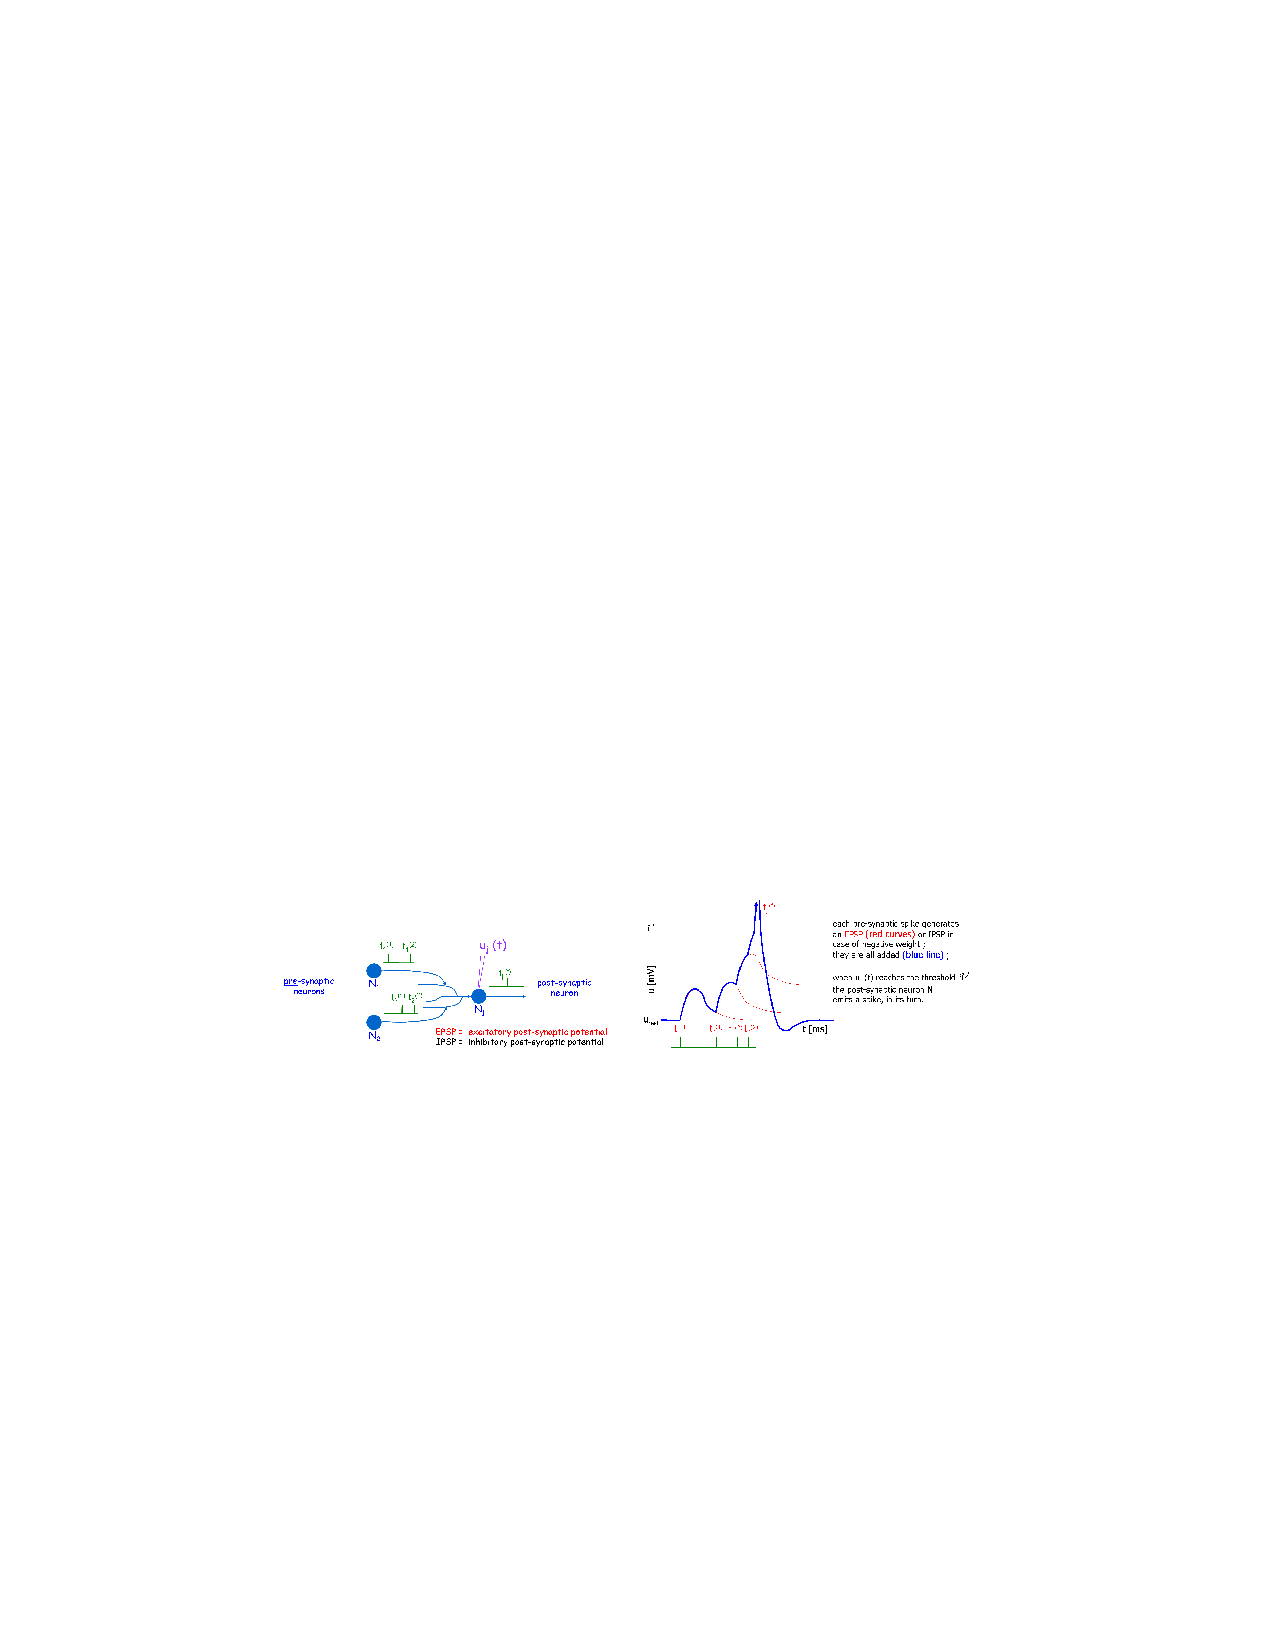
\includegraphics[width=1\linewidth]{image/SRM.pdf}
            \end{figure}

        \end{frame}
%---------------------------------------------------
		\begin{frame}
		  \frametitle{\textbf{Encoding and Decoding}}
            \begin{columns}
            \begin{column}{0.5\textwidth}
            \begin{figure}[h]
            \centering
            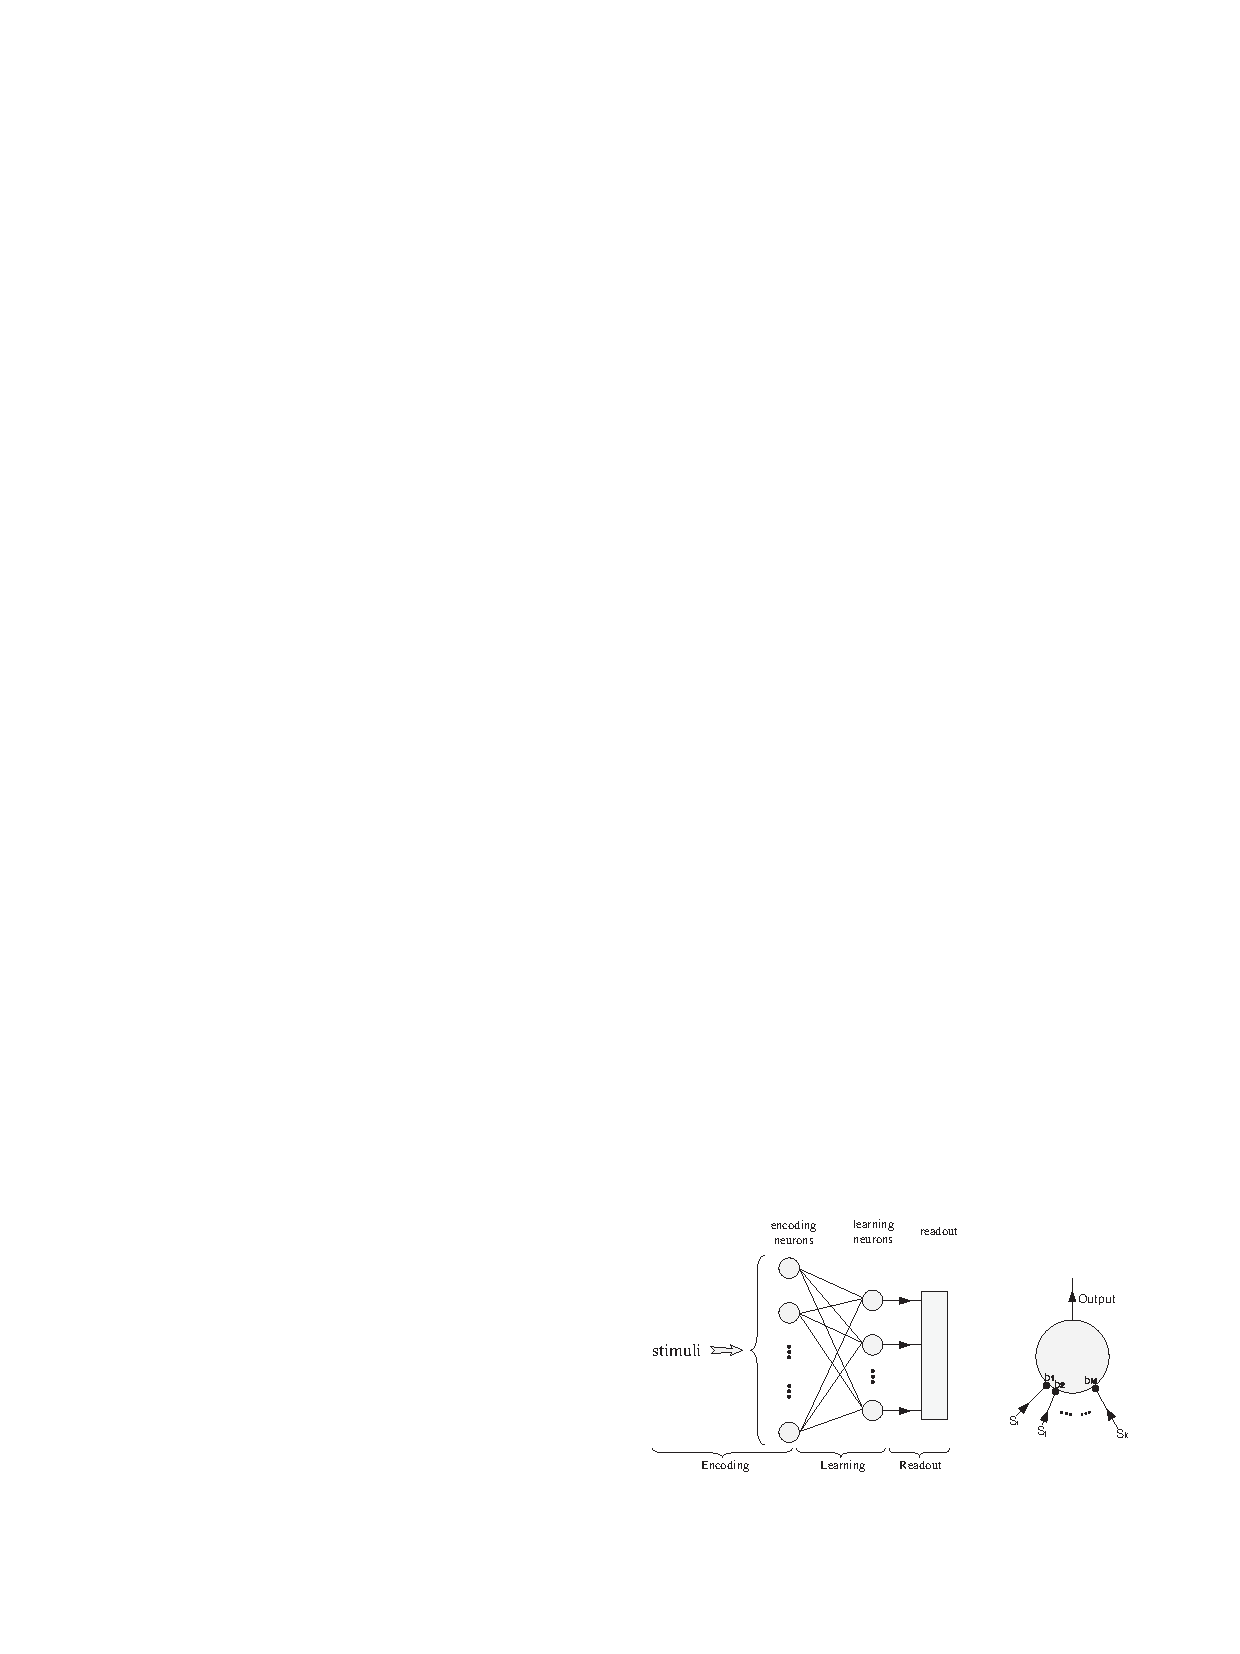
\includegraphics[width=1\linewidth]{image/Coding_2.pdf}
            \end{figure}
            \end{column}
            \begin{column}{0.5\textwidth}
            Encoding : P(response | stimulus)
            Decoding : P(stimulus | response)


            \end{column}
            \end{columns}
            \begin{figure}[h]
            \centering
            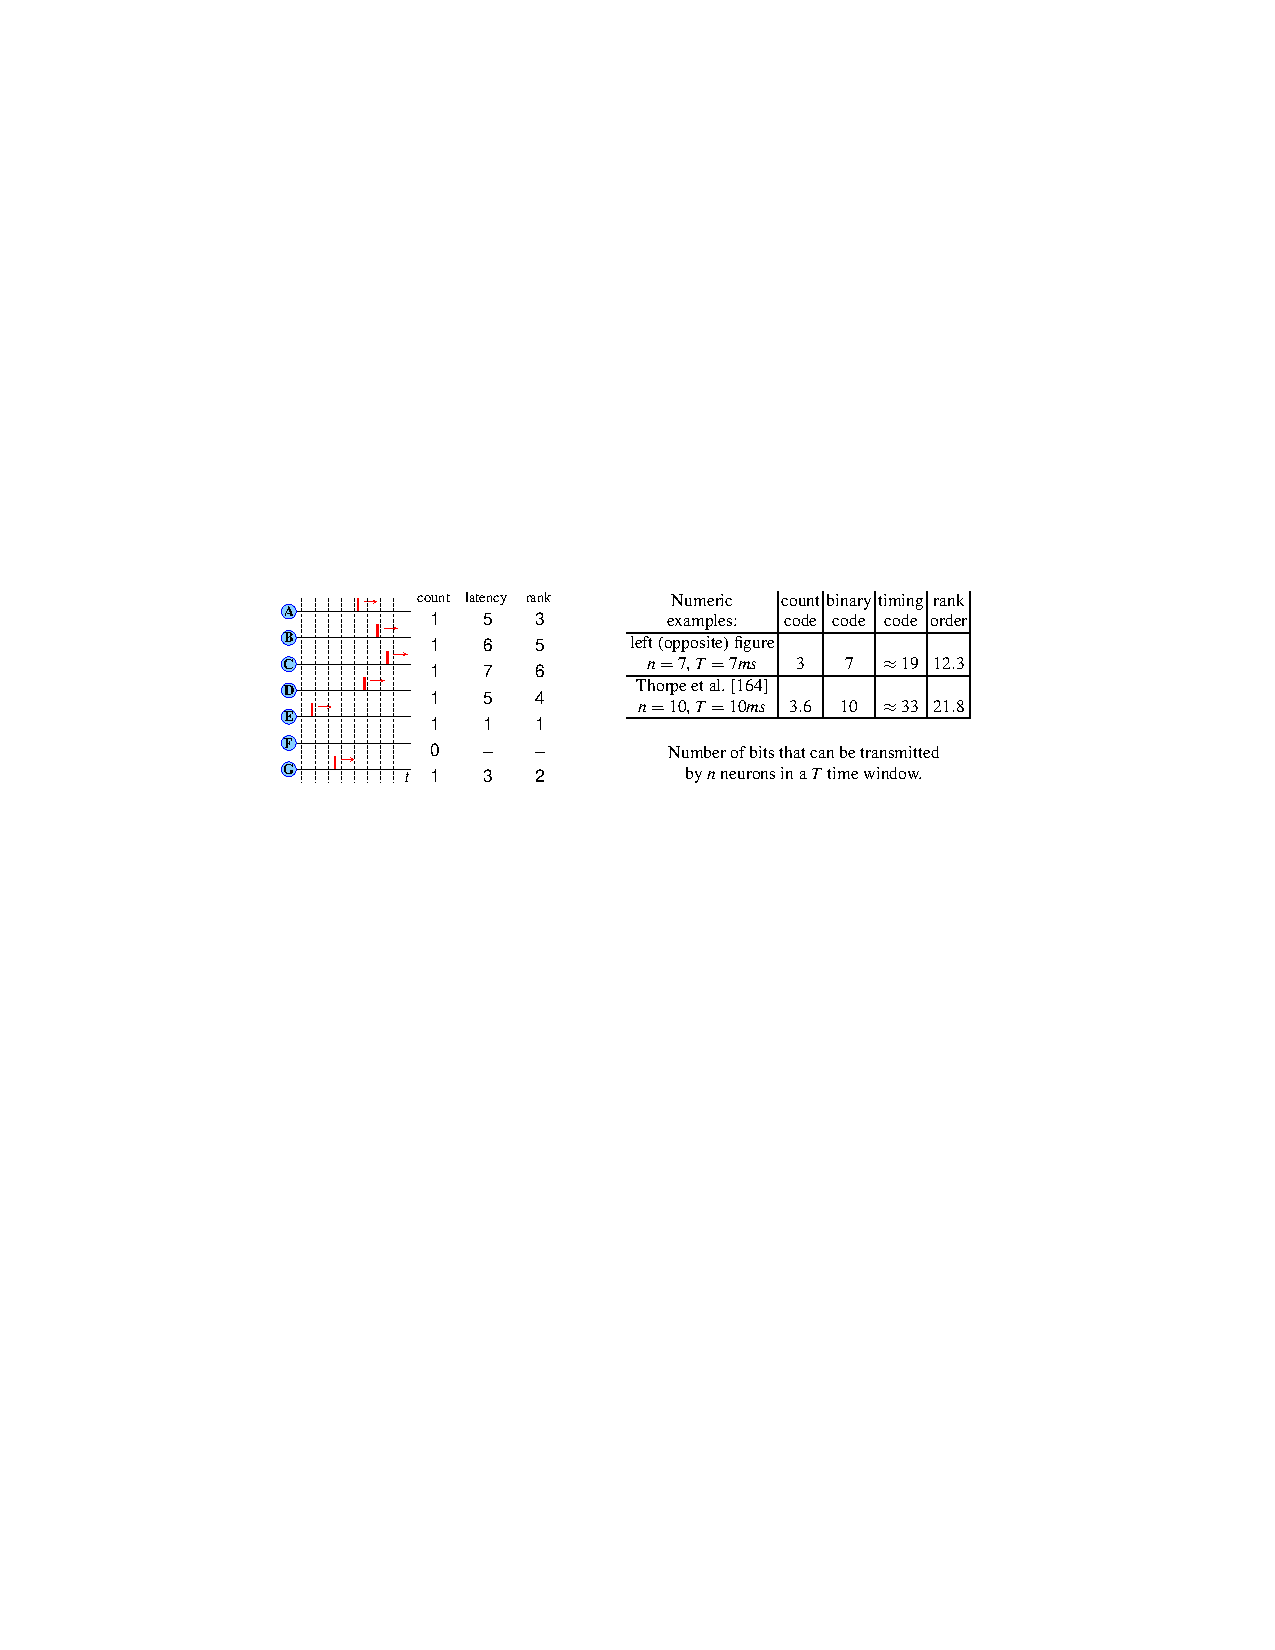
\includegraphics[width=0.8\linewidth]{image/Coding.pdf}
            \end{figure}
		\end{frame}

%---------------------------------------------------
        \begin{frame}
		  \frametitle{\textbf{Liquid State Machine}}
            \only<1>{\noindent\textbf{Liquid State Machine(LSM)} has emerged as a computational model that is more adequate than the Turing machine for \textcolor[rgb]{1.00,0.00,0.00}{describing computations in biological networks of neurons}. LSM is a model for real-time computations on \textcolor[rgb]{1.00,0.00,0.00}{continuous streams of data}.\cite{RN179,RN82}}
            \only<2>{\noindent {
            \begin{itemize}
              \item A layer of K neurons with \textbf{input connections} toward the reservoir.
              \item A \textcolor[rgb]{1.00,0.00,0.00}{recurrent network} of M neurons, interconnected by a random and \textcolor[rgb]{1.00,0.00,0.00}{sparse} set of weighted links: the so-called reservoir, that is usually left \textcolor[rgb]{1.00,0.00,0.00}{untrained}.
              \item A layer of L \textcolor[rgb]{1.00,0.00,0.00}{readout neurons} with trained connections from the reservoir.
            \end{itemize}
            }}
            \begin{figure}[h]
            \centering
            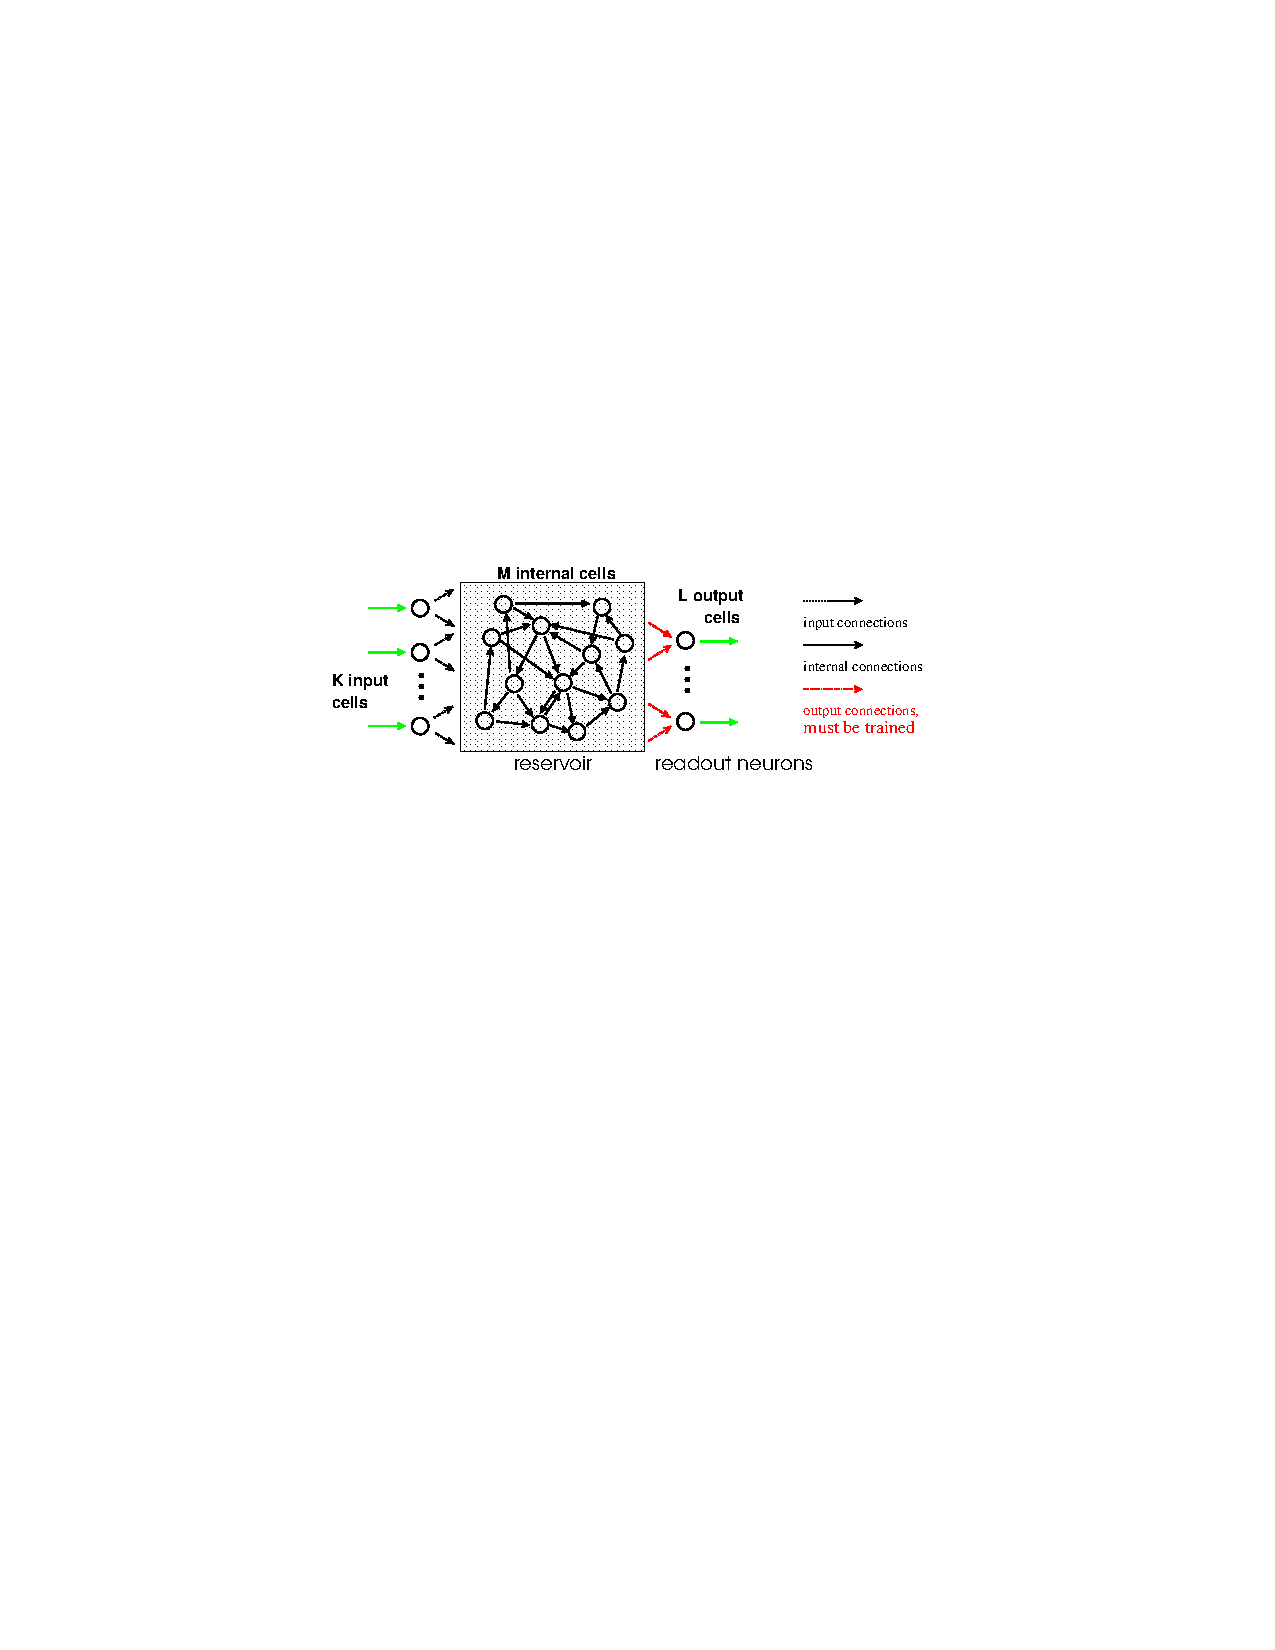
\includegraphics[width=0.9\linewidth]{image/LSM.pdf}
            \end{figure}
		\end{frame}
%---------------------------------------------------
		\begin{frame}
		  \frametitle{\textbf{Synaptic Plasticity}}
		    \begin{block}{\textbf{Spiking-Timing Dependent Plasticity(STDP)}}
            \begin{equation}
                \Delta w = \left\{
                            \begin{array}{lr}
                             A_+exp(-\Delta t/\tau_+) \quad if \Delta t\geq 0\\
                            \\
                            -A_-exp(-\Delta t/\tau_-) \quad if \Delta t < 0
                            \end{array}
                            \right.
            \end{equation}
            \end{block}

            \begin{columns}
            \begin{column}{0.4\textwidth}
            \begin{figure}[h]
            \centering
            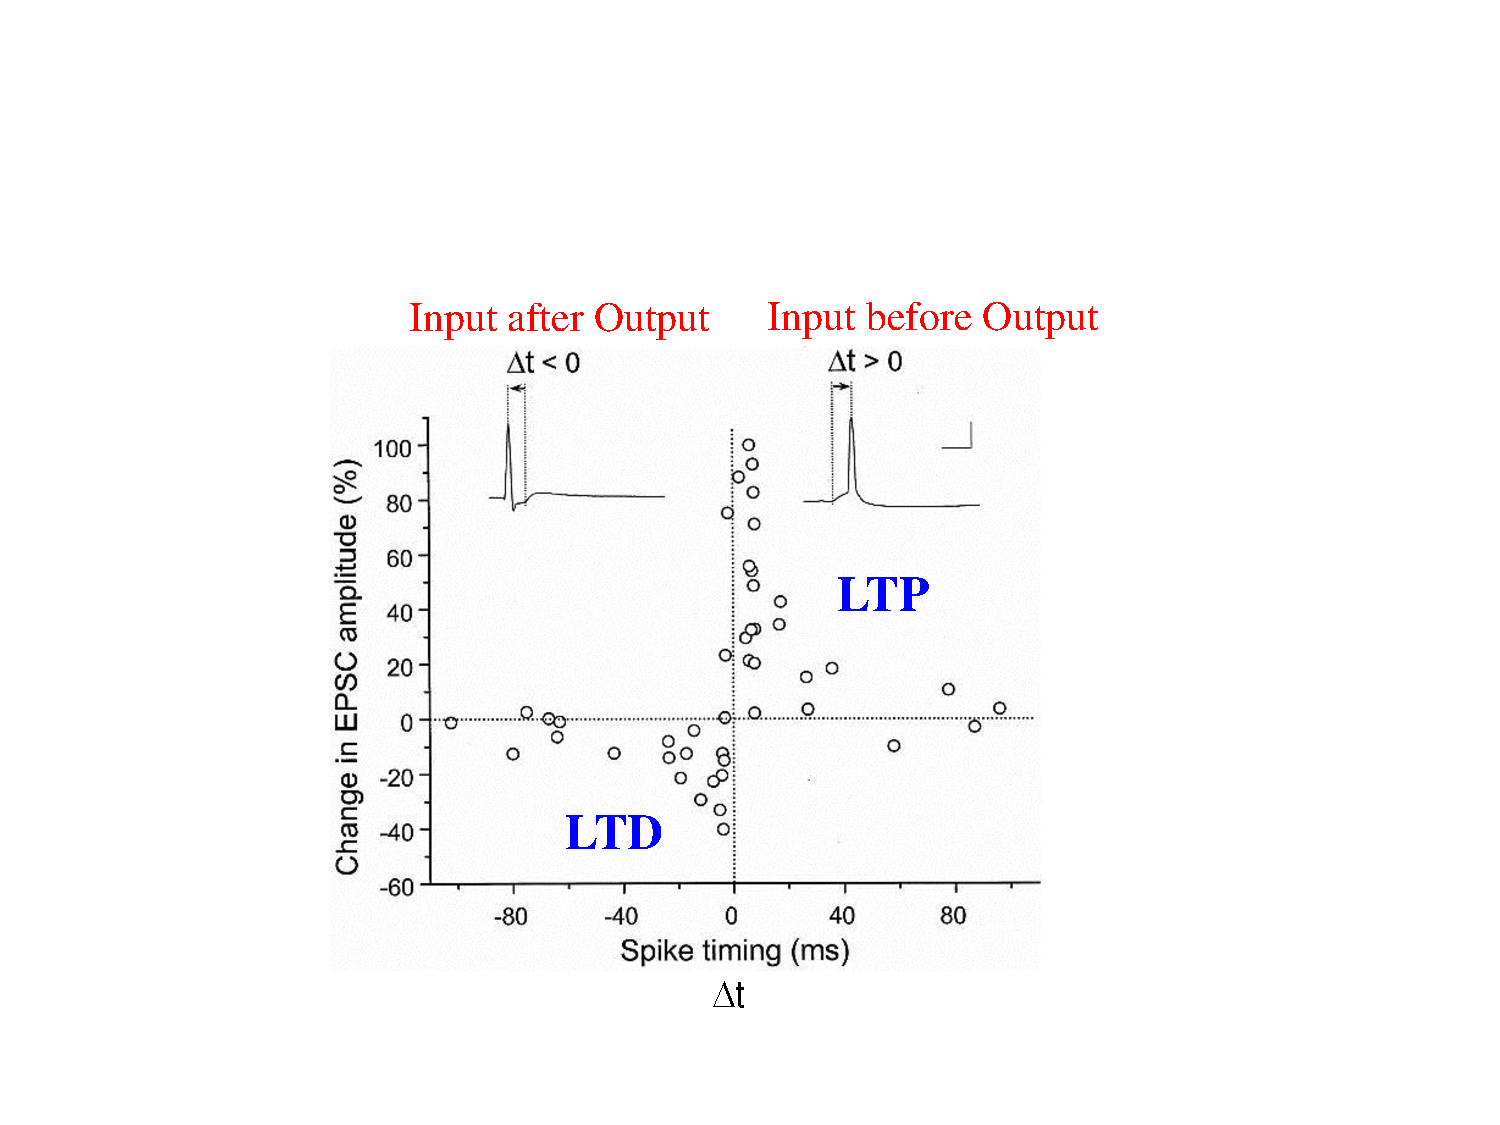
\includegraphics[width=1\linewidth]{image/STDP.pdf}
            \end{figure}
            \end{column}
            \begin{column}{0.5\textwidth}
            \begin{figure}[h]
            \centering
            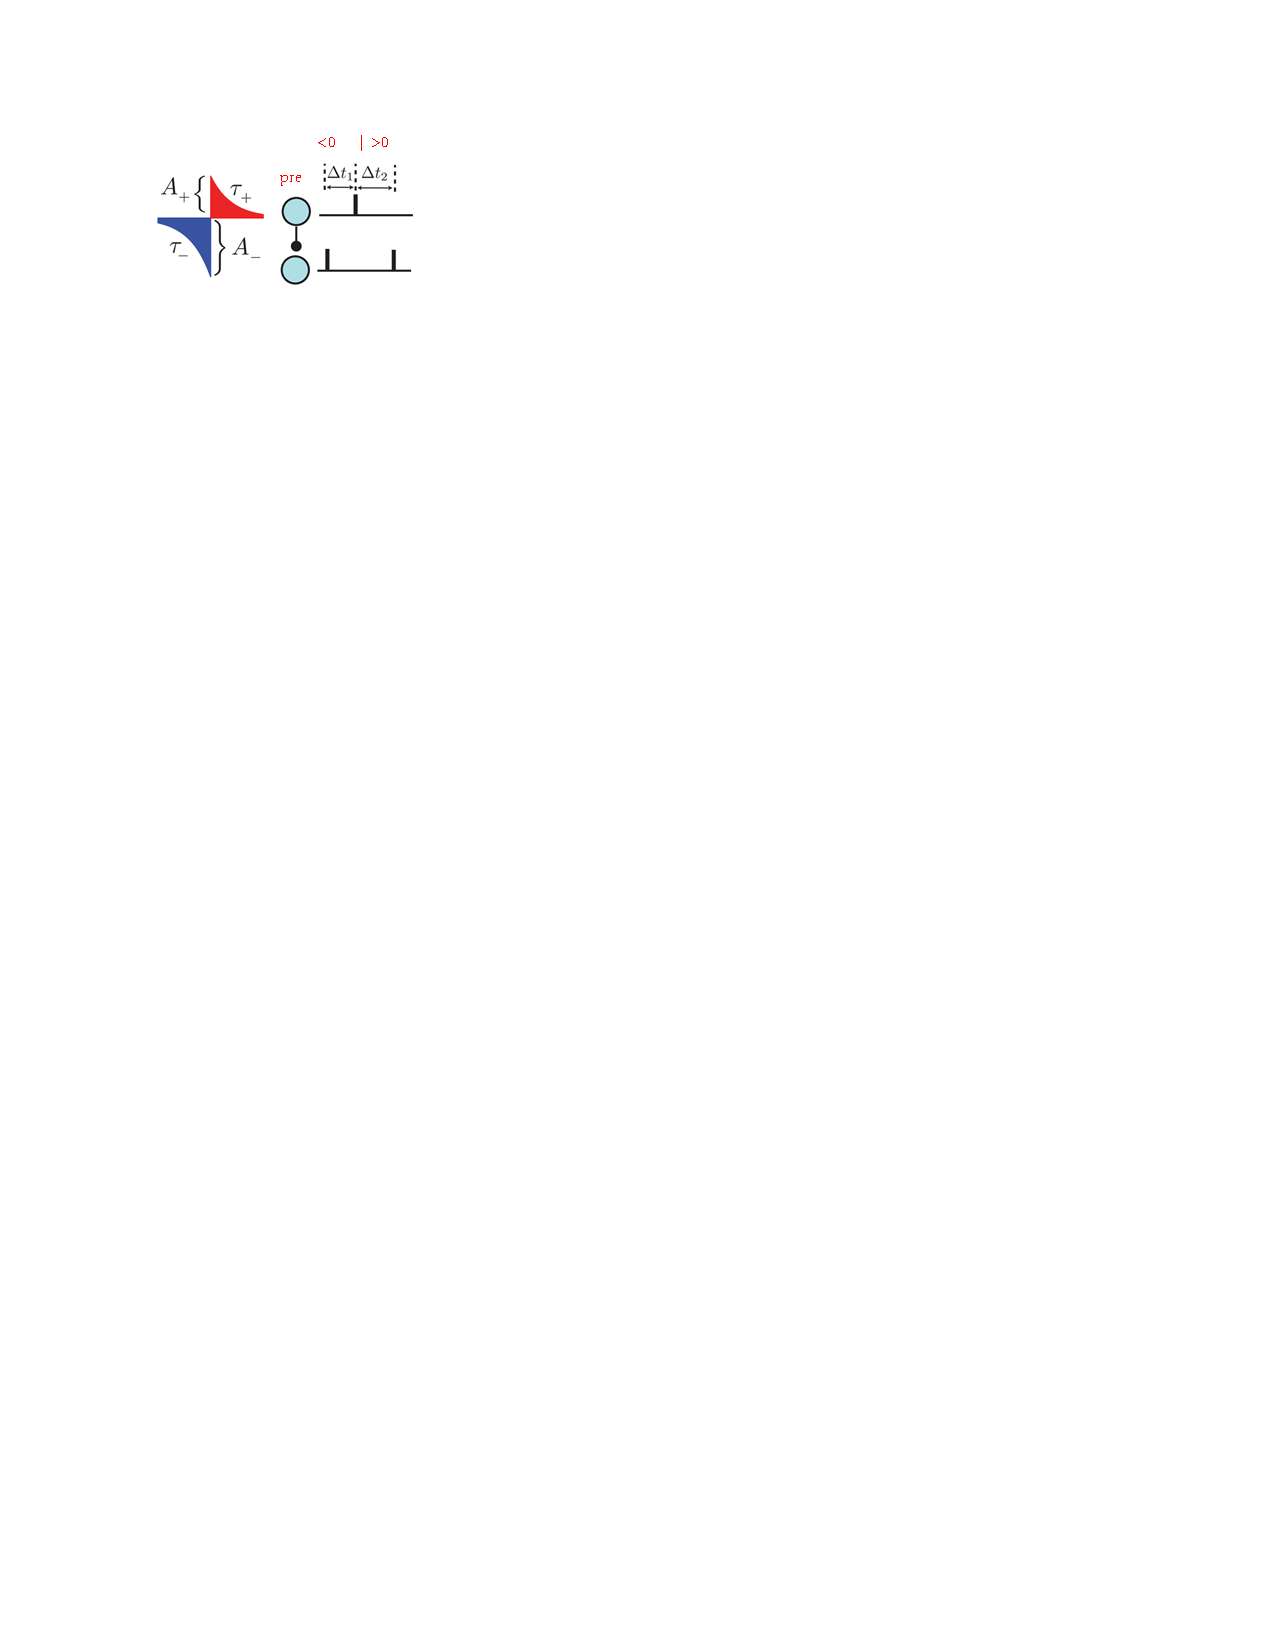
\includegraphics[width=1\linewidth]{image/STDP_2.pdf}
            \end{figure}
            \end{column}
            \end{columns}
		\end{frame}

\section[Algorithms]{Training LSM and Pattern Interference}
%---------------------------------------------------
		\begin{frame}
		  \frametitle{\textbf{Synaptic Competition in STDP}}
            \noindent Synaptic Competition is the significant mechanism of plasticity. The post-synaptic neurons have greater opportunity to response the spiking pattern of the winner in pre-synaptic neuron.\cite{RN172}
            \begin{figure}[htb]
            \centering
            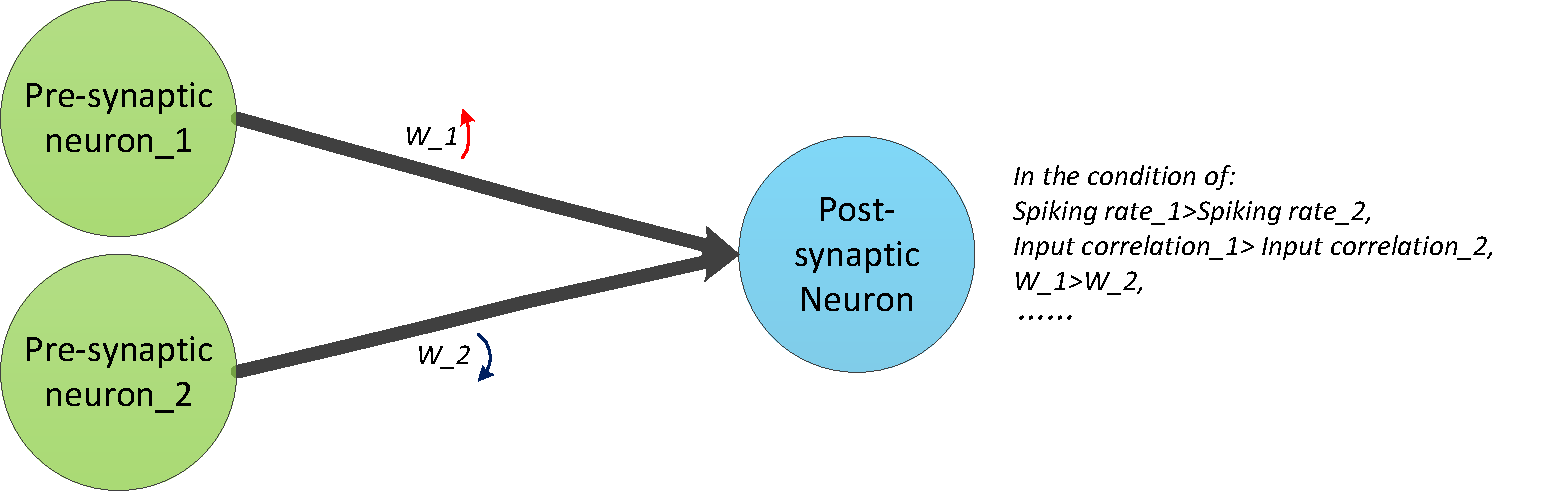
\includegraphics[width=0.9\linewidth]{image/synaptic_competition.pdf}
            \caption{Synaptic Competition in Neural Plasticity}
            \label{Competition_1}
            \end{figure}
		\end{frame}

		\begin{frame}
		  \frametitle{\textbf{Synaptic Competition in STDP}}
            \begin{figure}[htb]
            \centering
            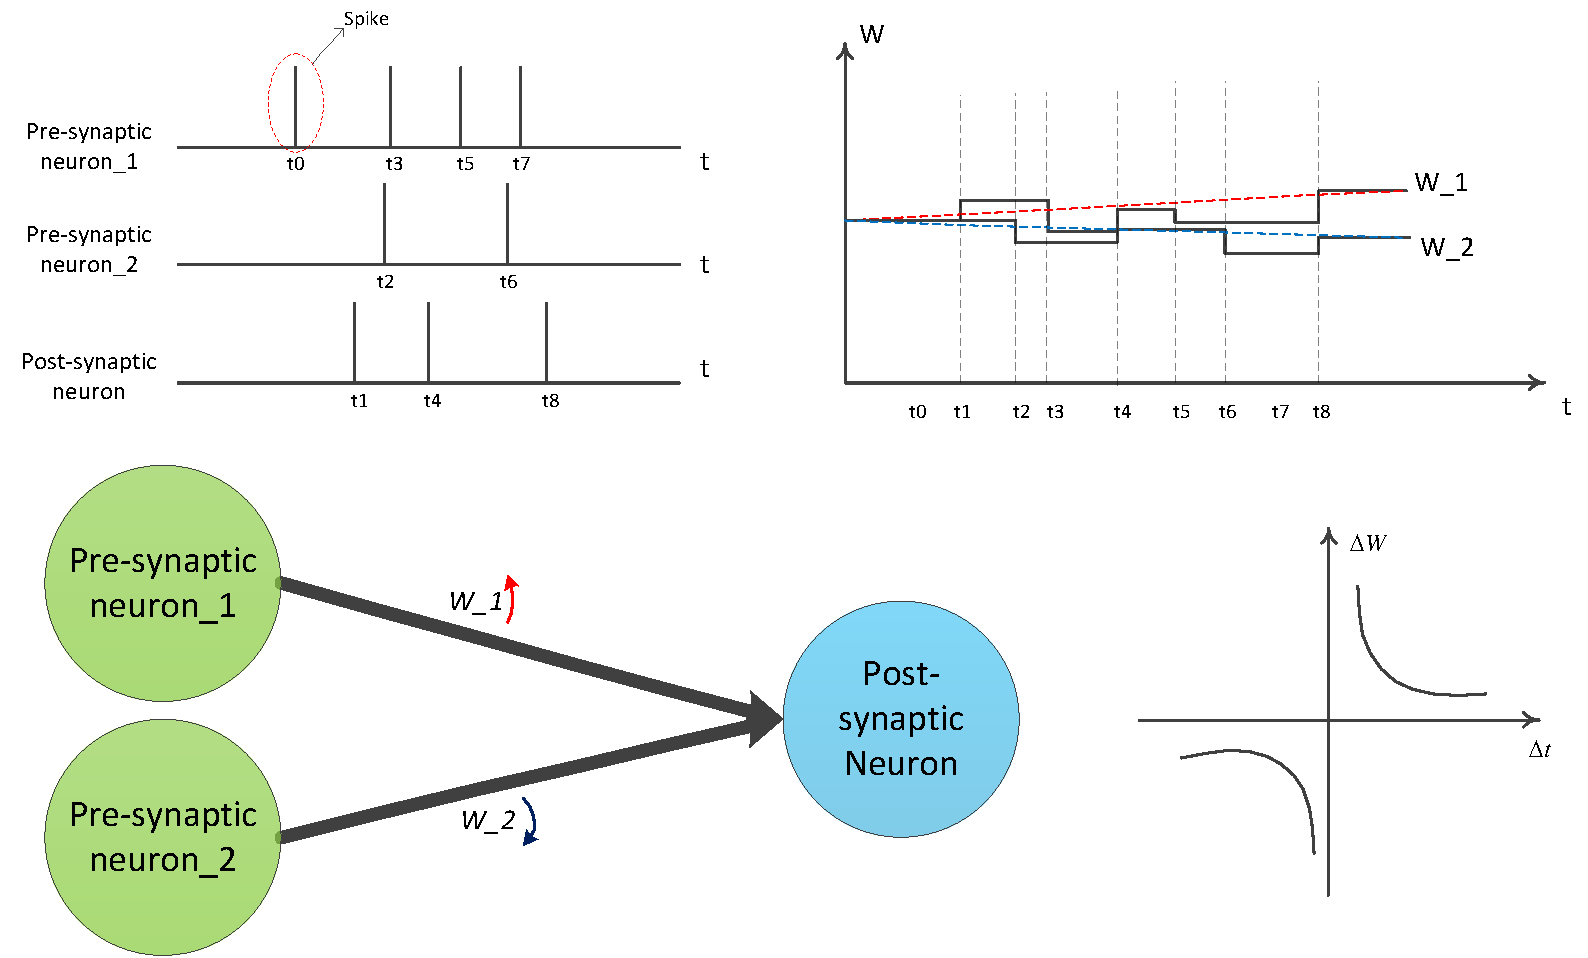
\includegraphics[width=0.9\linewidth]{image/illustration_competition.pdf}
            \caption{Illustration of Competition in Neural Plasticity}
            \label{Competition_2}
            \end{figure}
		\end{frame}

		\begin{frame}
		  \frametitle{\textbf{Separative Responses in Reservoir}}
            \begin{figure}[htb]
            \centering
            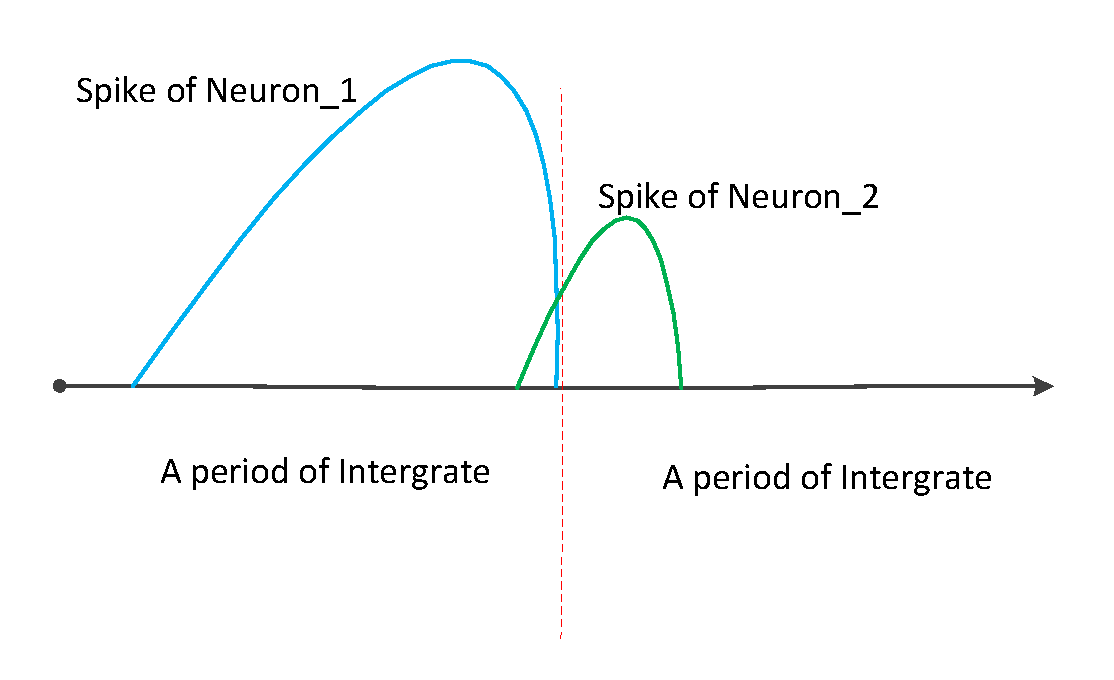
\includegraphics[width=0.9\linewidth]{image/Separative_Responses_in_Reservoir.pdf}
            \caption{Illustration of Separative Responses in Reservoir}
            \label{Separative_R_2}
            \end{figure}            		
		\end{frame}

		\begin{frame}
		  \frametitle{\textbf{Training internal synapses of Reservoir with STDP}}
		    \begin{figure}[htb]
            \centering
            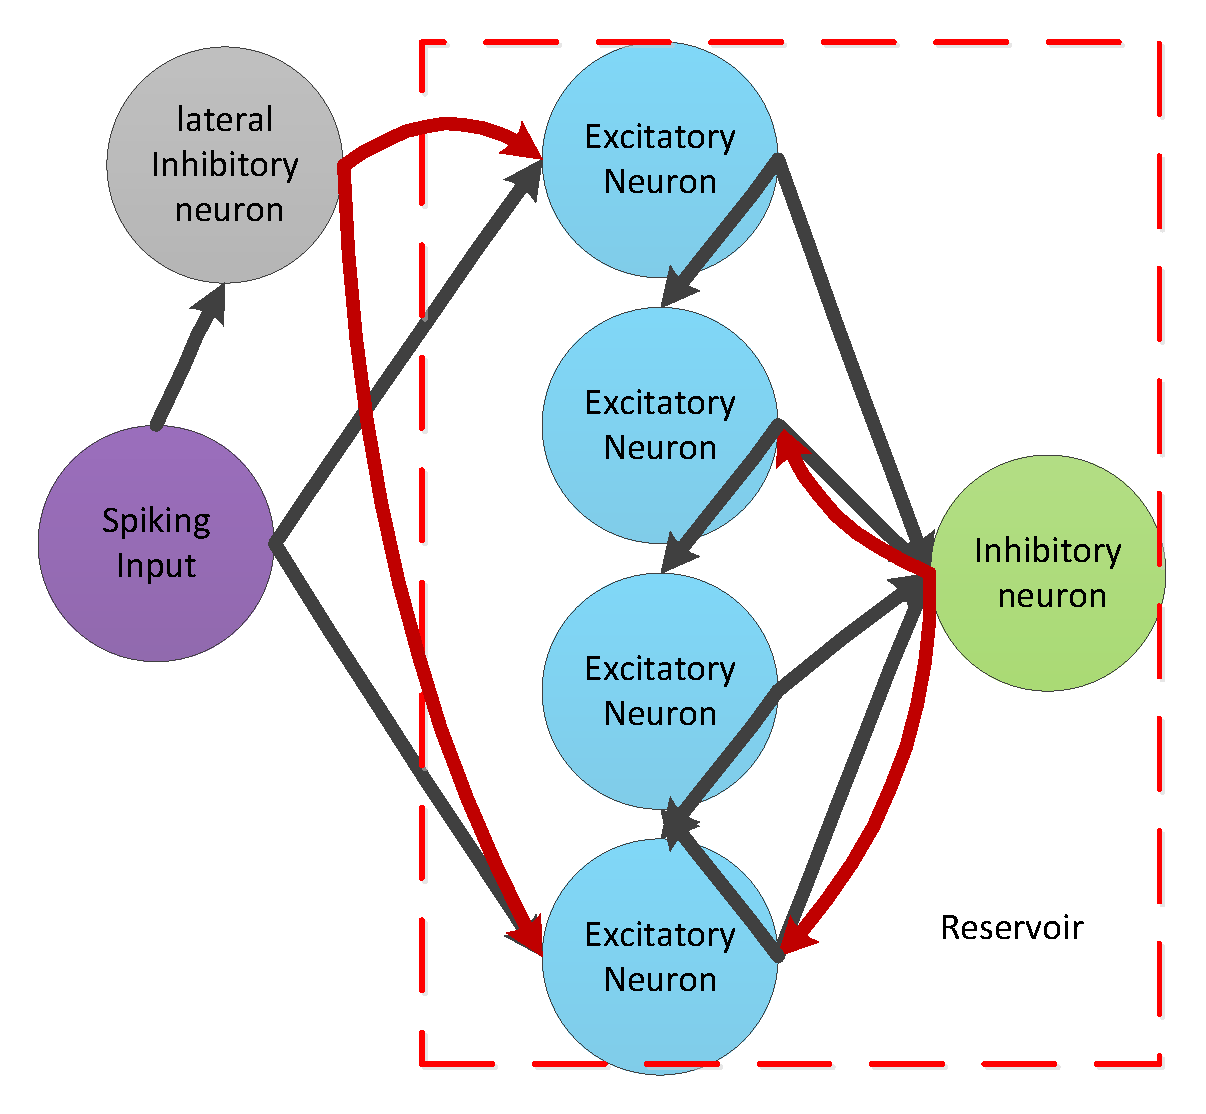
\includegraphics[width=0.6\linewidth]{image/LSM_model.pdf}
            \caption{LSM model with lateral inhibitory neuron}
            \label{Separative_R_2}
            \end{figure}
		\end{frame}

%		\begin{frame}
%		  \frametitle{\textbf{Interference between patterns in Synaptic Plasticity}}
%		
%		\end{frame}
\section[Results]{Results for Benchmark Testing}
%---------------------------------------------------
		\begin{frame}
		  \frametitle{\textbf{Spike Trains classification}}
		  \framesubtitle{Simulations Setting}
            \begin{columns}
            \begin{column}{0.5\textwidth}
            \begin{figure}[h]
            \centering
            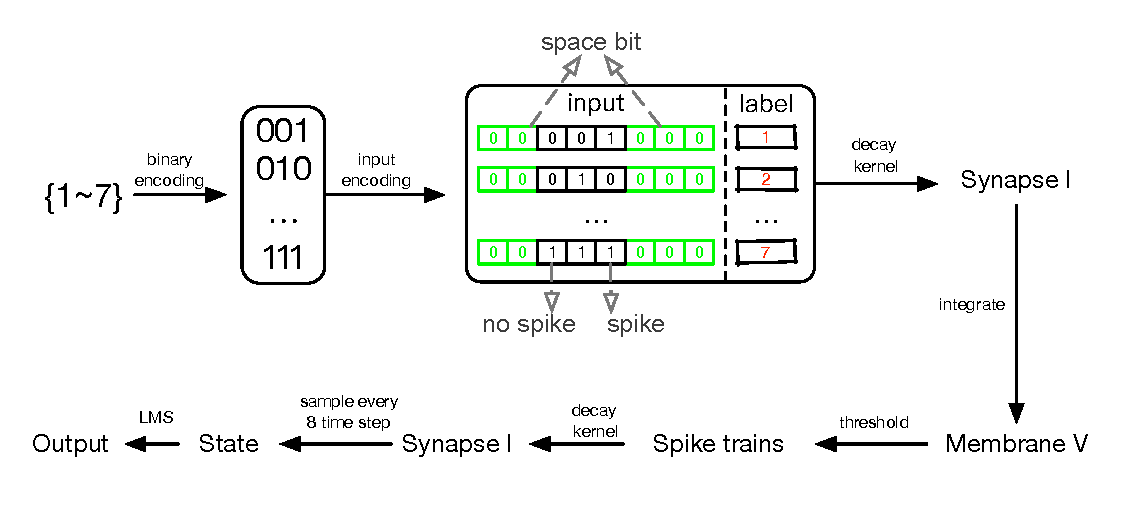
\includegraphics[width=0.9\linewidth]{image/sim2.pdf}
            \caption{Spike Trains Classification}
            \label{ST_Task}
            \end{figure}
            \end{column}
            \begin{column}{0.5\textwidth}
            \noindent {Patterns:}\\
                \small { [[1, 1, 1, 1, 1, 0, 0, 0, 0, 0],

                         [1, 1, 0, 1, 1, 0, 0, 1, 0, 1],

                         [1, 0, 1, 1, 0, 0, 1, 0, 1, 0],

                         [0, 1, 0, 1, 0, 1, 0, 1, 0, 1],

                         [0, 0, 1, 1, 0, 0, 1, 0, 1, 0],

                         [0, 1, 0, 1, 1, 0, 1, 1, 0, 1],

                         [0, 1, 1, 1, 0, 0, 1, 1, 1, 0],

                         [0, 1, 1, 0, 1, 0, 1, 0, 1, 1],

                         [1, 1, 0, 0, 1, 0, 1, 1, 1, 0],

                         [1, 0, 1, 1, 0, 1, 0, 0, 0, 1]]}
            \end{column}
            \end{columns}
		\end{frame}
%---------------------------------------------------
		\begin{frame}
		  \frametitle{\textbf{Spike Trains classification}}
		  \framesubtitle{Results}
            \begin{columns}
            \begin{column}{0.5\textwidth}
            \begin{figure}[h]
            \centering
            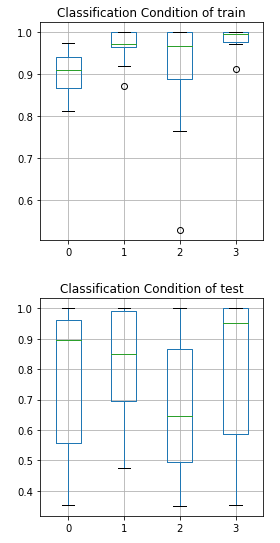
\includegraphics[width=0.5\linewidth]{image/ST_without_stdp_party.png}
            \caption{Statistics AUC for 10 simulations in ST classification without STDP}
            \label{ST_Task}
            \end{figure}
            \end{column}
            \begin{column}{0.5\textwidth}
            \begin{figure}[h]
            \centering
            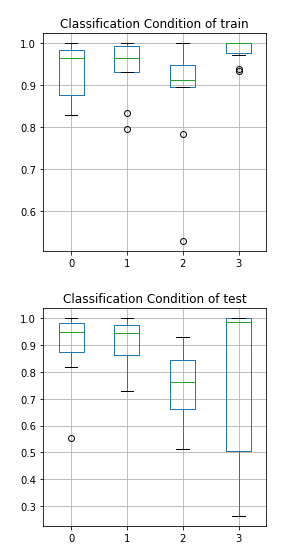
\includegraphics[width=0.5\linewidth]{image/ST_with_stdp_party.png}
            \caption{Statistics AUC for 10 simulations in ST classification with STDP}
            \label{ST_Task}
            \end{figure}
            \end{column}
            \end{columns}
		\end{frame}
%---------------------------------------------------
		\begin{frame}
		  \frametitle{\textbf{Tri-function classification}}
		  \framesubtitle{Simulations Setting}
            \begin{columns}
            \begin{column}{0.5\textwidth}
            The task is to predict which of three signal generating functions is currently active in producing a varying input signal. To generate a sample of the signal at a given timestep, one of the three following function types is used.
            \end{column}
            \begin{column}{0.5\textwidth}
           \begin{figure}[h]
            \centering
            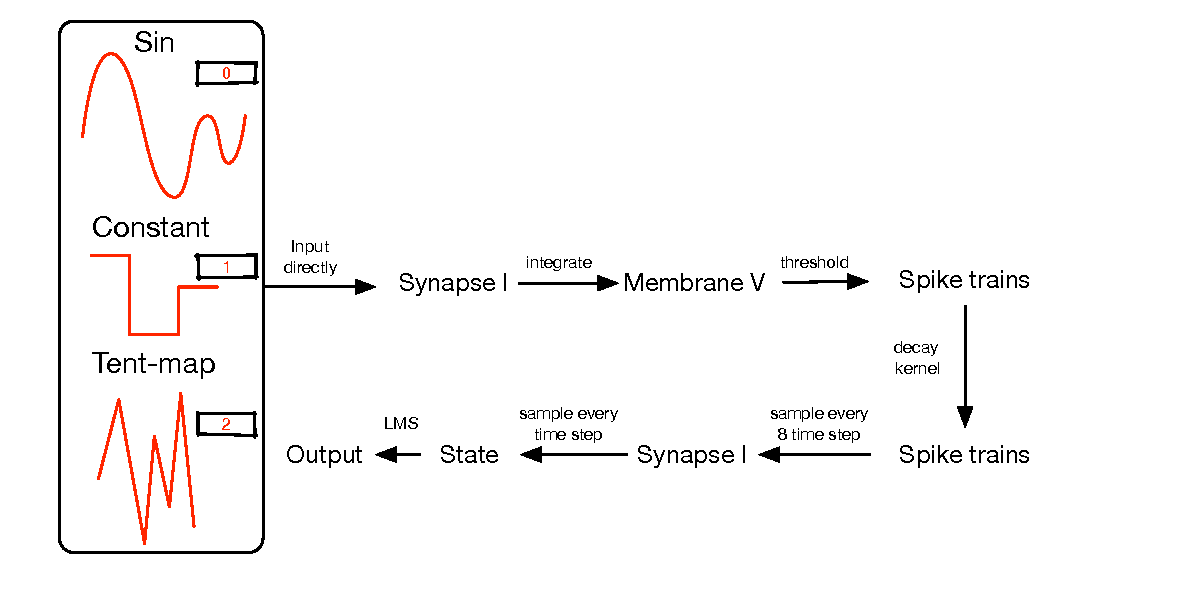
\includegraphics[width=1.0\linewidth]{image/sim3.pdf}
            \caption{Tri-function Classification}
            \label{Tri_Task}
            \end{figure}
            \end{column}
            \end{columns}
           \begin{figure}[h]
            \centering
            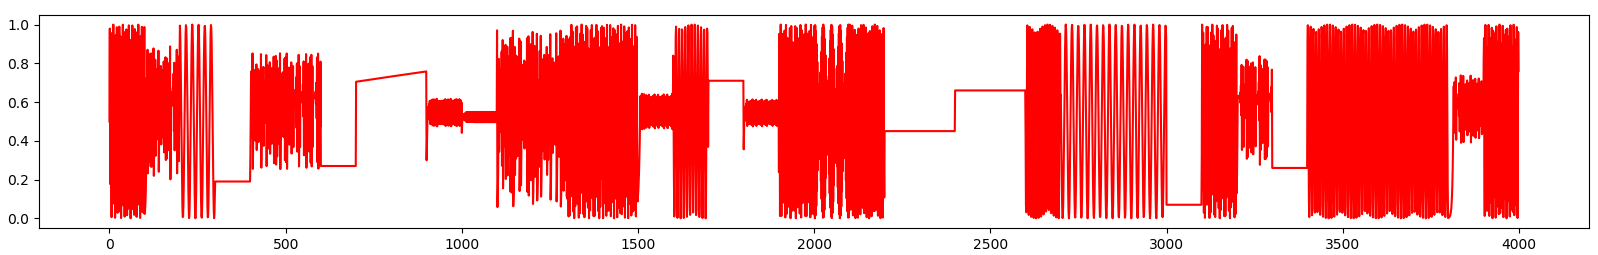
\includegraphics[width=0.9\linewidth]{image/Tri_data.png}
            \caption{Spike Trains Classification}
            \label{Tri_Data}
            \end{figure}
		\end{frame}
%---------------------------------------------------
		\begin{frame}
		  \frametitle{\textbf{Tri-function classification}}
		  \framesubtitle{Results}
            \begin{columns}
            \begin{column}{0.5\textwidth}
            \begin{figure}[h]
            \centering
            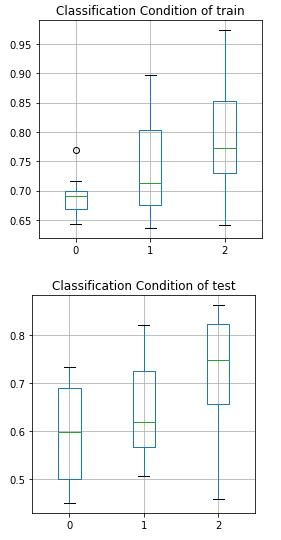
\includegraphics[width=0.5\linewidth]{image/Tri_without_stdp.png}
            \caption{Statistics AUC for 10 simulations in Tri classification without STDP}
            \label{ST_Task}
            \end{figure}
            \end{column}
            \begin{column}{0.5\textwidth}
            \begin{figure}[h]
            \centering
            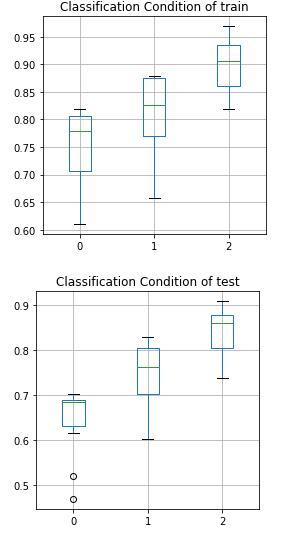
\includegraphics[width=0.5\linewidth]{image/Tri_with_stdp.png}
            \caption{Statistics AUC for 10 simulations in Tri classification with STDP}
            \label{ST_Task}
            \end{figure}
            \end{column}
            \end{columns}
		\end{frame}
%---------------------------------------------------
%		\begin{frame}
%		  \frametitle{\textbf{Japanese Vowels classification}}
%		  \framesubtitle{}
%
%		\end{frame}

\section[Discussion]{Discussion}
%---------------------------------------------------
		\begin{frame}
		  \frametitle{\textbf{\secname}}
		    \begin{itemize}
                \item Training LSM is difficult due to the complicated recurrent structure.
                \item The primary hyper-parameter is the integral time constant $\tau$, which should be suitable for the classification task.
                \item STDP can only change the synaptic weights, but the structure is fixed before training reservoir. In this case, the ability of STDP is limited.
            \end{itemize}
		    \end{frame}
%%---------------------------------------------------
%\begin{frame}{Note test}
%  \begin{itemize}
%     \item<1-> Eggs
%     \item<2-> Plants
%       \note[item]<2>{Tell joke about plants.}
%  \end{itemize}
%\end{frame}

\small\section*{Bibliography}
%----------------------------------------------------------------------
\begin{frame}[allowframebreaks]\frametitle{\secname}
\frametitle{Bibliography}
\bibliographystyle{plain}
\bibliography{reference}
\end{frame}

\section*{}
%---------------------------------------------------
            \begin{frame}

                \begin{center}
                    \begin{minipage}{1\textwidth}
                        \setbeamercolor{mybox}{fg=white, bg=frametitle.bg}
                        \begin{beamercolorbox}[wd=0.70\textwidth, rounded=true, shadow=true]{mybox}
                        \LARGE \centering Thanks for Listening
                        \LARGE \centering and
                        \LARGE \centering Questions?
                        \end{beamercolorbox}
                    \end{minipage}
                \end{center}

                \begin{center}
                    \begin{minipage}{1\textwidth}
                        \setbeamercolor{mybox}{fg=white, bg=white!20!frametitle.bg}
                        \begin{beamercolorbox}[wd=0.90\textwidth, rounded=true, shadow=true]{mybox}
                        \small \textbf{Download:} \textcolor[rgb]{0.00,0.00,1.00}{\underline{\url{https://pan.baidu.com/s/1htmMfOC}}} Password:ad8j
                        \end{beamercolorbox}
                    \end{minipage}
                \end{center}

                \begin{columns}
                    \pgfputat{\pgfxy(-1.0,-6.5)}{\pgfbox[left,bottom]{\pgfimage[width=0.5cm,height=0.5cm]{figures/brian-logo.png}}}
                    \pgfputat{\pgfxy(-0.5,-6.5)}{\pgfbox[left,bottom]{\pgfimage[width=0.5cm,height=0.5cm]{figures/jupyter.png}}}
                    \pgfputat{\pgfxy(0.0,-6.5)}{\pgfbox[left,bottom]{\pgfimage[width=0.5cm,height=0.5cm]{figures/github.png}}}
                    \pgfputat{\pgfxy(0.5,-6.5)}{\pgfbox[left,bottom]{\pgfimage[width=0.75cm,height=0.5cm]{figures/latex.png}}}
                    \pgfputat{\pgfxy(1.25,-6.5)}{\pgfbox[left,bottom]{\pgfimage[width=0.5cm,height=0.5cm]{figures/matplotlib_med.png}}}
                    \pgfputat{\pgfxy(1.75,-6.5)}{\pgfbox[left,bottom]{\pgfimage[width=0.75cm,height=0.5cm]{figures/numpy_logo.png}}}
                    \pgfputat{\pgfxy(2.5,-6.5)}{\pgfbox[left,bottom]{\pgfimage[width=2cm,height=0.5cm]{figures/pandas_logo.png}}}
                    \pgfputat{\pgfxy(4.5,-6.5)}{\pgfbox[left,bottom]{\pgfimage[width=1.75cm,height=0.5cm]{figures/Vmware_logo.png}}}
                    \pgfputat{\pgfxy(6.25,-6.5)}{\pgfbox[left,bottom]{\pgfimage[width=0.5cm,height=0.5cm]{figures/python.jpg}}}
                    \pgfputat{\pgfxy(6.75,-6.5)}{\pgfbox[left,bottom]{\pgfimage[width=1cm,height=0.5cm]{figures/scikit-learn-logo-small.png}}}
                    \pgfputat{\pgfxy(7.75,-6.5)}{\pgfbox[left,bottom]{\pgfimage[width=0.5cm,height=0.5cm]{figures/scipy_med.png}}}
                    \pgfputat{\pgfxy(8.25,-6.5)}{\pgfbox[left,bottom]{\pgfimage[width=0.5cm,height=0.5cm]{figures/teamview.jpg}}}
                    \pgfputat{\pgfxy(8.75,-6.5)}{\pgfbox[left,bottom]{\pgfimage[width=0.5cm,height=0.5cm]{figures/pycharm.jpg}}}
                \end{columns}

            \end{frame}

\end{document}
